\documentclass{beamer}
\usetheme{default}
\usecolortheme{seahorse}
\usepackage[utf8]{inputenc}
\usepackage{graphicx}
\usepackage{booktabs}
\usepackage{amsmath}
\usepackage{natbib}
\usepackage[english]{babel}
\usepackage{hyphenat}
\usepackage{tikz}
\usetikzlibrary{shapes,arrows.meta,positioning}

\title[Lecture 5]{A Bit of SEM}
\subtitle{Advanced Master in Agricultural Economics and Policy}
\author{Giovanbattista Califano}
\date[Portici, 30/04/2026]{Attitudinal Scales for the Study \\ of Consumer Preferences \\ April 30, 2026}
\institute[UNINA]{University of Naples Federico II, giovanbattista.califano@unina.it}

\tikzset{
  lv/.style = {draw=blue!80, fill=blue!10, very thick, ellipse, minimum height=1cm, minimum width=2cm, align=center},
  mv/.style = {draw=blue!80, fill=blue!10, very thick, rectangle, minimum height=0.5cm, minimum width=1cm, align=center},
  ev/.style = {draw=blue!80, fill=blue!10, very thick, circle, minimum size=0.6cm, inner sep=1pt, align=center},
  arrow/.style = {thick, ->, >=Stealth}
}

\AtBeginSection[]
{
  \begin{frame}<beamer>
    \frametitle{Moving on to...}
    \tableofcontents[currentsection]
  \end{frame}
}

\begin{document}

\frame{\titlepage}

\begin{frame}{Roadmap}
    \begin{center}
        \begin{tabular}{|l|l|c|}
        \hline
        20/04 &  Hello, Psychometrics! & $\checkmark$ \\
        \hline
        23/04 &  The Questionnaire & $\checkmark$ \\
        \hline
        24/04 & Reliability and Validity of a Measure & $\checkmark$ \\
        \hline
        27/04 & Latent Variables: Reflective or Formative? & $\checkmark$ \\
        \hline
        30/04 & A Bit of SEM & $\bigcirc$ \\
        \hline
        07/05 & Stata Stata Stata Stata Stata Stata Stata & $\bigcirc$ \\
        \hline
        \end{tabular}
    \end{center}
\vspace{0.1cm}
\footnotesize
Recommended readings: \\
\begin{itemize}
    \item Chapters 4 and 7 from \cite{jhangiani2019research}
    \item Chapters 7, 10 and 14 from \cite{olivero2022psicologia}
    \item Chapter 12 from \cite{mehmetoglu2022applied}
\end{itemize}
\scriptsize
\bibliographystyle{apalike}
\bibliography{text}
\end{frame}

\begin{frame}{Before we begin...}
    \centering
    \url{https://www.stata.com/manuals/sem.pdf}
\end{frame}

\begin{frame}{Before we begin...}
    \begin{figure}
        \centering
        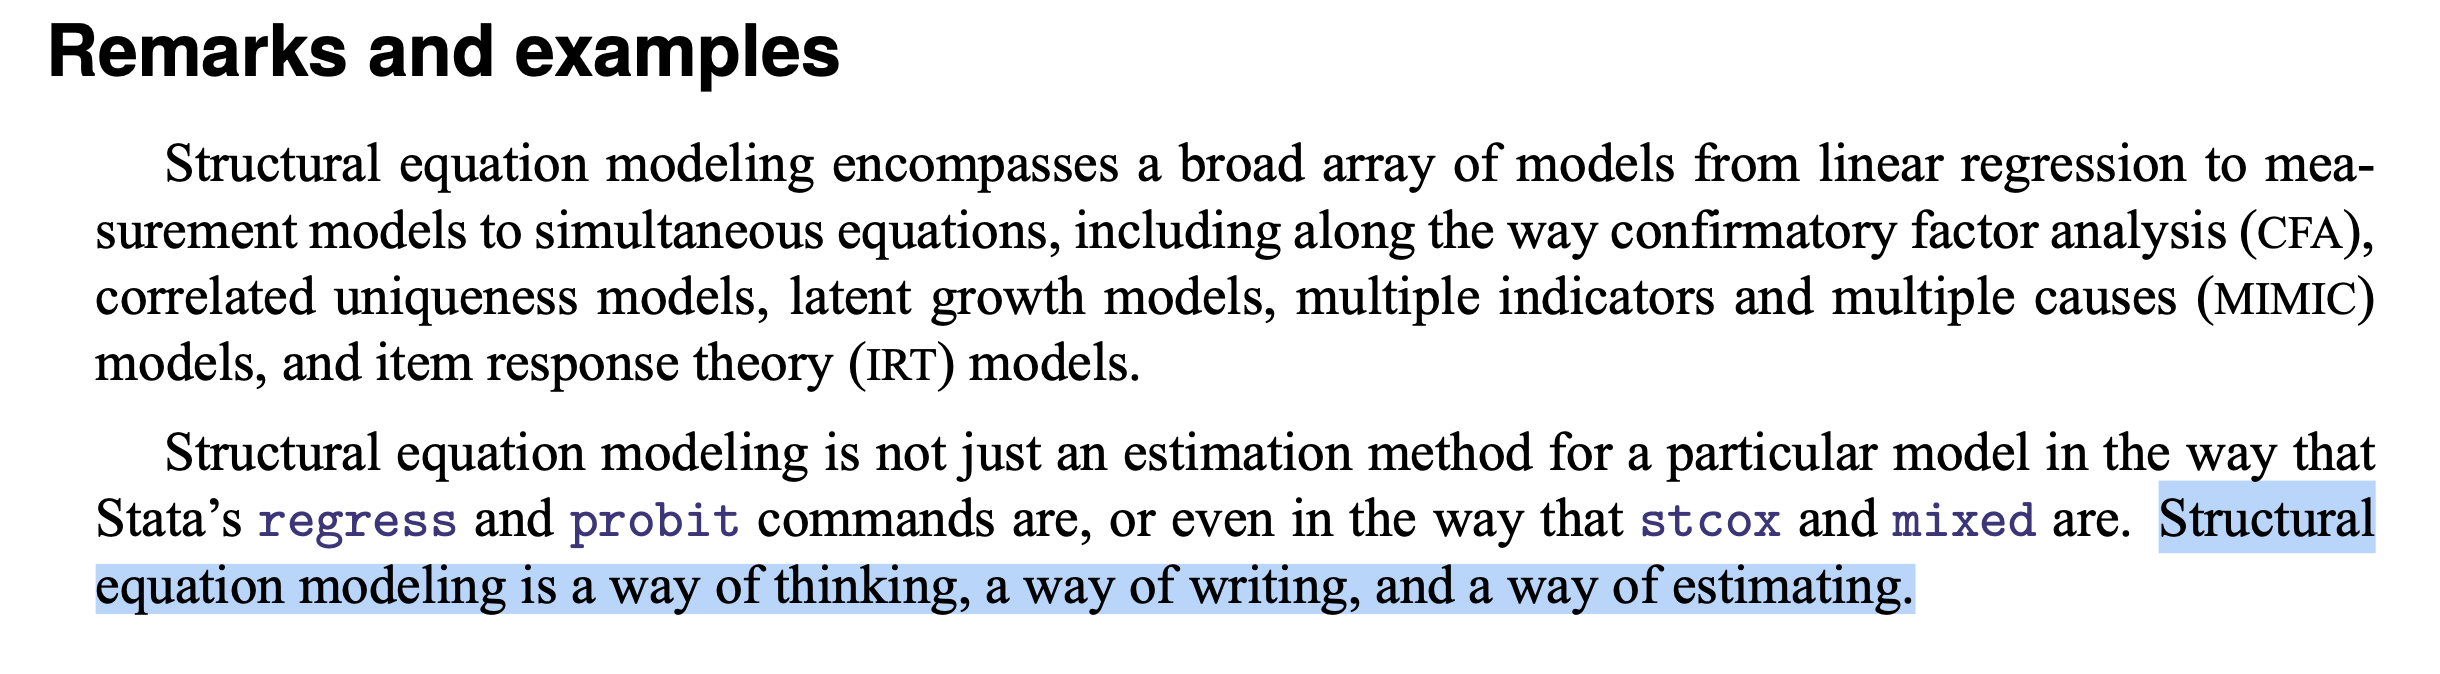
\includegraphics[width=1\linewidth]{manual.png}
    \end{figure}
    \centering
    \pause
    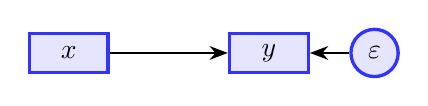
\begin{tikzpicture}[node distance=0.3 and 1.5, auto]
        \node[mv] (x) {$x$};
        \node[mv, right=of x] (y) {$y$};
        \node[ev, right=0.5 of y] (e) {$\varepsilon$};
        \draw[arrow] (x) -- (y);
        \draw[arrow] (e) -- (y);
    \end{tikzpicture}
\end{frame}

\begin{frame}{Before we begin...}
    \begin{figure}
        \centering
        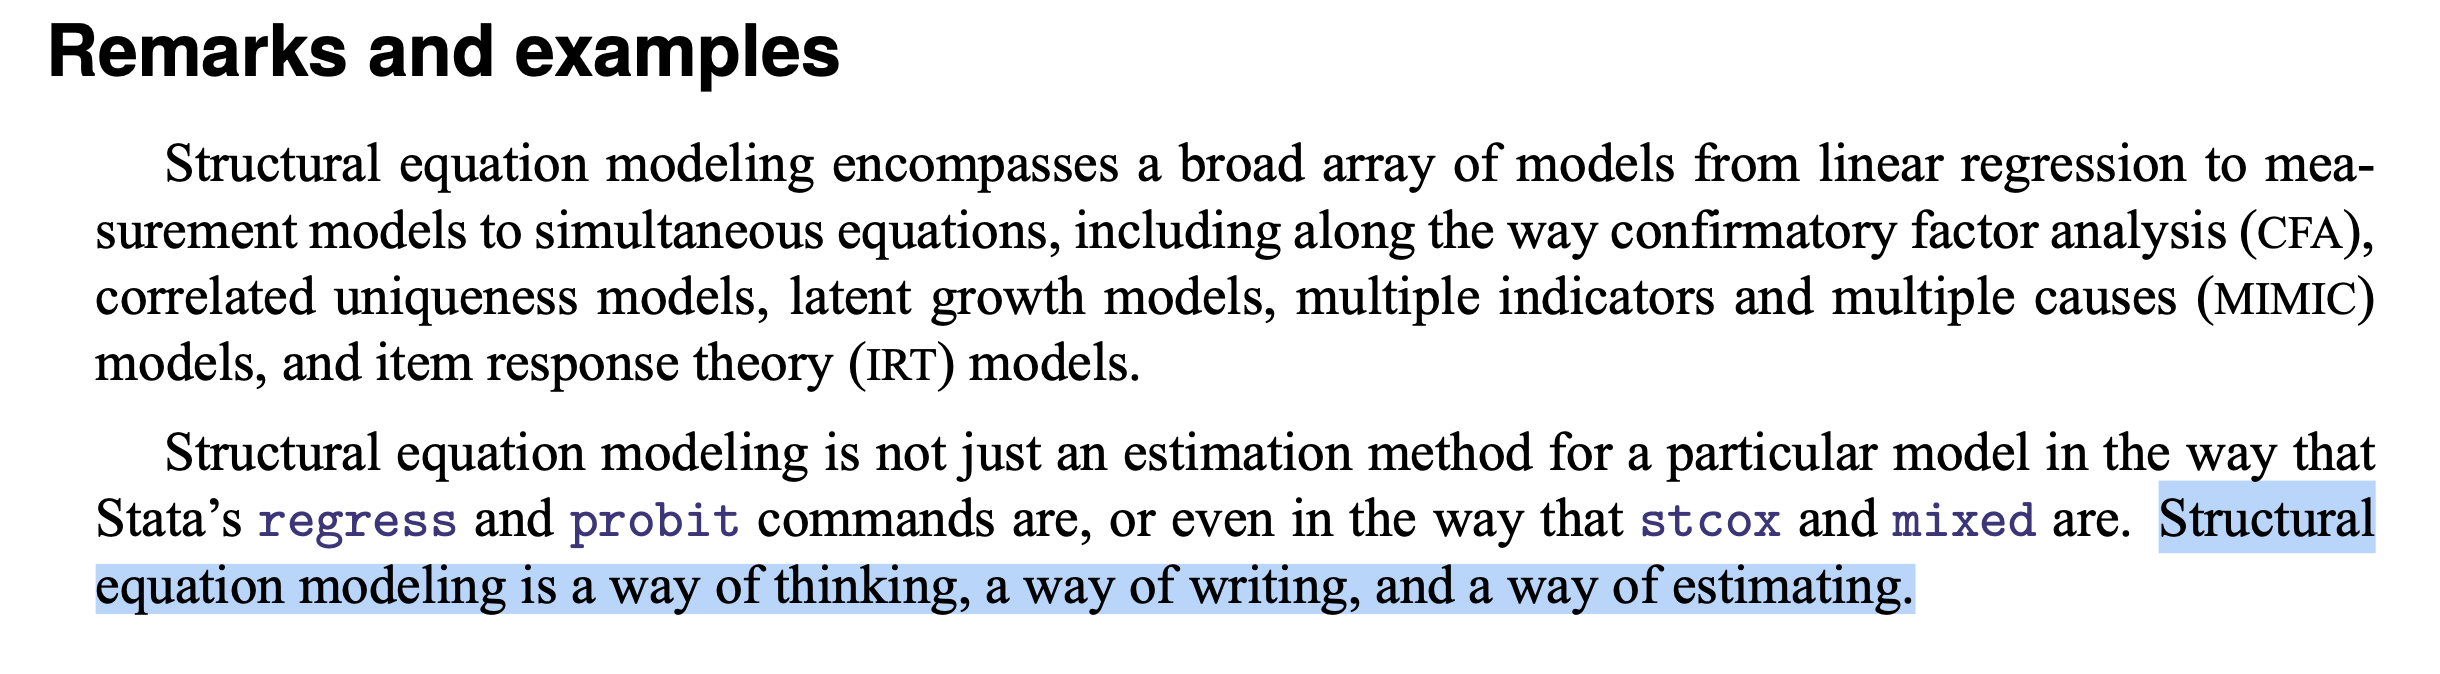
\includegraphics[width=1\linewidth]{manual.png}
    \end{figure}
    \centering
    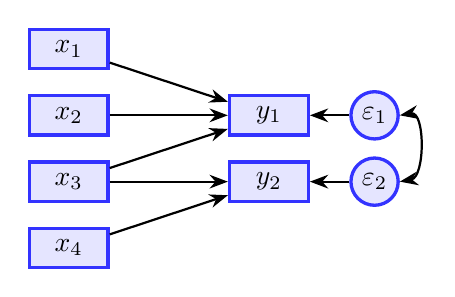
\begin{tikzpicture}[node distance=0.3 and 1.5, auto]
        \node[mv] (x1) {$x_1$};
        \node[mv, below=of x1] (x2) {$x_2$};
        \node[mv, below=of x2] (x3) {$x_3$};
        \node[mv, below=of x3] (x4) {$x_4$};
        \node[mv, right=of x2] (y1) {$y_1$};
        \node[mv, right=of x3] (y2) {$y_2$};
        \node[ev, right=0.5 of y1] (e1) {$\varepsilon_1$};
        \node[ev, right=0.5 of y2] (e2) {$\varepsilon_2$};
        \draw[arrow] (x1) -- (y1);
        \draw[arrow] (x2) -- (y1);
        \draw[arrow] (x3) -- (y1);
        \draw[arrow] (x3) -- (y2);
        \draw[arrow] (x4) -- (y2);
        \draw[arrow] (e1) -- (y1);
        \draw[arrow] (e2) -- (y2);
        \draw[<->, thick, >=Stealth] (e1.east) to [out=10,in=10] (e2.east);
    \end{tikzpicture}
\end{frame}

\section{A Bit of Terminology}
\begin{frame}{Types of SEM}
    \begin{itemize}
        \item Structural equation modelling allows us to estimate relationships between observed and/or latent variables through the study of the variance-covariance matrix. For this reason, it is also called \textbf{Covariance Based (CB) SEM}\footnote{Also to distinguish it from Partial Least Squares (PLS) SEM.}.
        \item Since it is used to estimate multiple equations simultaneously, models are described and reported in the form of block diagrams.
        \item As the Stata manual also noted, under the umbrella of SEM fall many different models...
    \end{itemize}
\end{frame}

\begin{frame}{Some examples}
    \centering
    \textbf{Path Analysis (PA)} \\
    \vspace{2em}
    \begin{columns}
        \column{0.5\textwidth}
        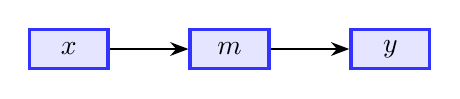
\begin{tikzpicture}
            \node[mv] (y) {$y$};
            \node[mv, left=of y] (m) {$m$};
            \node[mv, left=of m] (x) {$x$};
            \draw[arrow] (x) -- (m);
            \draw[arrow] (m) -- (y);
        \end{tikzpicture}
        \column{0.5\textwidth}
        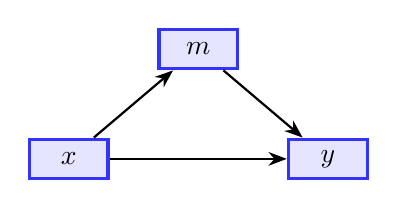
\begin{tikzpicture}
            \node[mv] (y) {$y$};
            \node[left=of y] (dummy) {};
            \node[mv, above=of dummy] (m) {$m$};
            \node[mv, left=of dummy] (x) {$x$};
            \draw[arrow] (x) -- (m);
            \draw[arrow] (m) -- (y);
            \draw[arrow] (x) -- (y);
        \end{tikzpicture}
    \end{columns}
    \vspace{2em}
    \textit{Relationships between manifest variables are estimated.}
\end{frame}

\begin{frame}{Some examples}
    \centering
    \textbf{Path Analysis (PA)} \\
    \vspace{2em}
        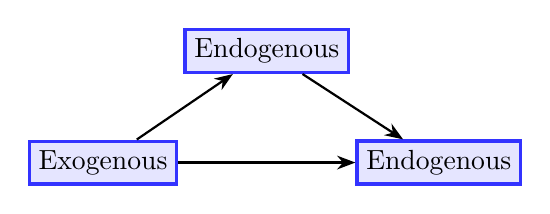
\begin{tikzpicture}
            \node[mv] (y) {Endogenous};
            \node[left=of y] (dummy) {};
            \node[mv, above=of dummy] (m) {Endogenous};
            \node[mv, left=of dummy] (x) {Exogenous};
            \draw[arrow] (x) -- (m);
            \draw[arrow] (m) -- (y);
            \draw[arrow] (x) -- (y);
        \end{tikzpicture}
    \vspace{2em}
    \textit{In these models it is complicated to speak of dependent and independent variables. Variables that are not explained within the model are called exogenous, while those that are explained are called endogenous.}
\end{frame}

\begin{frame}{Some examples}
    \centering
    \textbf{Confirmatory Factor Analysis (CFA)} \\
    \vspace{2em}
        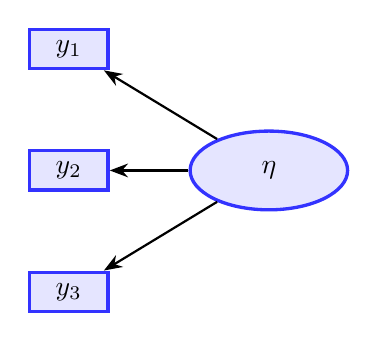
\begin{tikzpicture}
            \node[lv] (l) {$\eta$};
            \node[mv, left=of l] (x2) {$y_2$};
            \node[mv, above=of x2] (x1) {$y_1$};
            \node[mv, below=of x2] (x3) {$y_3$};
            \draw[arrow] (l) -- (x1);
            \draw[arrow] (l) -- (x2);
            \draw[arrow] (l) -- (x3);
        \end{tikzpicture}
    \vspace{2em}
    \textit{Relationships between manifest and latent variables are estimated.}
\end{frame}

\begin{frame}{Some examples}
    \centering
    \textbf{Latent Path Analysis (LPA)} \\
    \vspace{2em}
        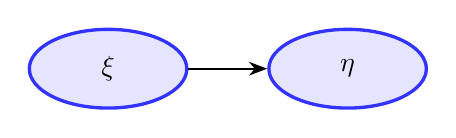
\begin{tikzpicture}
            \node[lv] (et) {$\eta$};
            \node[lv, left=of et] (xi) {$\xi$};
            \draw[arrow] (xi) -- (et);
        \end{tikzpicture}
    \vspace{2em}
    \textit{Relationships between latent variables are estimated.}
\end{frame}

\begin{frame}{Some examples}
    \centering
    \textbf{CFA + LPA} \\
    \textit{What is commonly meant by SEM} \\
    \vspace{2em}
        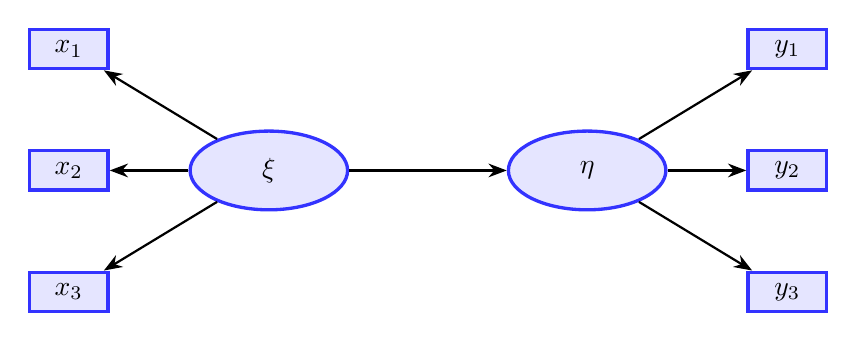
\begin{tikzpicture}
            \node[lv] (et) {$\eta$};
            \node[lv, left=2 of et] (xi) {$\xi$};
            \node[mv, left=of xi] (x2) {$x_2$};
            \node[mv, above=of x2] (x1) {$x_1$};
            \node[mv, below=of x2] (x3) {$x_3$};
            \node[mv, right=of et] (y2) {$y_2$};
            \node[mv, above=of y2] (y1) {$y_1$};
            \node[mv, below=of y2] (y3) {$y_3$};
            \draw[arrow] (xi) -- (et);
            \draw[arrow] (xi) -- (x1);
            \draw[arrow] (xi) -- (x2);
            \draw[arrow] (xi) -- (x3);
            \draw[arrow] (et) -- (y1);
            \draw[arrow] (et) -- (y2);
            \draw[arrow] (et) -- (y3);
        \end{tikzpicture}
    \vspace{2em}
    \small
    \textit{In these cases the CFA part is referred to as the \textbf{measurement model} or \textbf{outer model}. The LPA (or PA) part, on the other hand, is referred to as the \textbf{structural model} or \textbf{inner model}.}
\end{frame}

\begin{frame}{Some examples}
    \centering
    \textbf{Are latent variables only continuous?} \\
    \vspace{2em}
        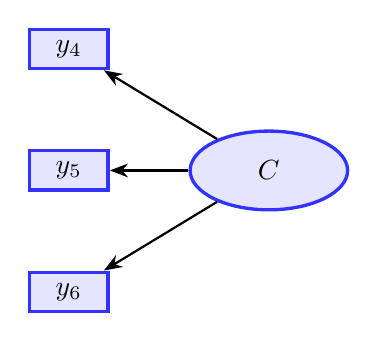
\begin{tikzpicture}
            \node[lv] (l) {$C$};
            \node[mv, left=of l] (x2) {$y_5$};
            \node[mv, above=of x2] (x1) {$y_4$};
            \node[mv, below=of x2] (x3) {$y_6$};
            \draw[arrow] (l) -- (x1);
            \draw[arrow] (l) -- (x2);
            \draw[arrow] (l) -- (x3);
        \end{tikzpicture}
    \vspace{2em}
    \textit{No. We can hypothesise the existence of unobservable (or unobserved) classes and estimate them from observed indicators. SEM with categorical latent variables include Latent Class Analysis, Latent Profile Analysis, and other finite mixture models.}
\end{frame}

\section{A Bit of History}
\begin{frame}{Brief history of SEM}
    \small
    \begin{block}{Origins}
        SEM analysis originates from the integration of:
        \begin{itemize}
            \item \textbf{Path Analysis} (Sewall Wright, 1921)
            \item \textbf{Factor Analysis} (Spearman, 1904; Thurstone, 1930)
            \item \textbf{Latent variable models} (Jöreskog, 1969)
        \end{itemize}
        \vspace{0.5em}
        SEM unifies causal and measurement approaches within a single statistical framework.
    \end{block}
    \begin{columns}[c]
    \column{0.25\textwidth}
    \begin{figure}
        \centering
        \footnotesize\textbf{Sewall Wright} \\
        \vspace{0.2em}
        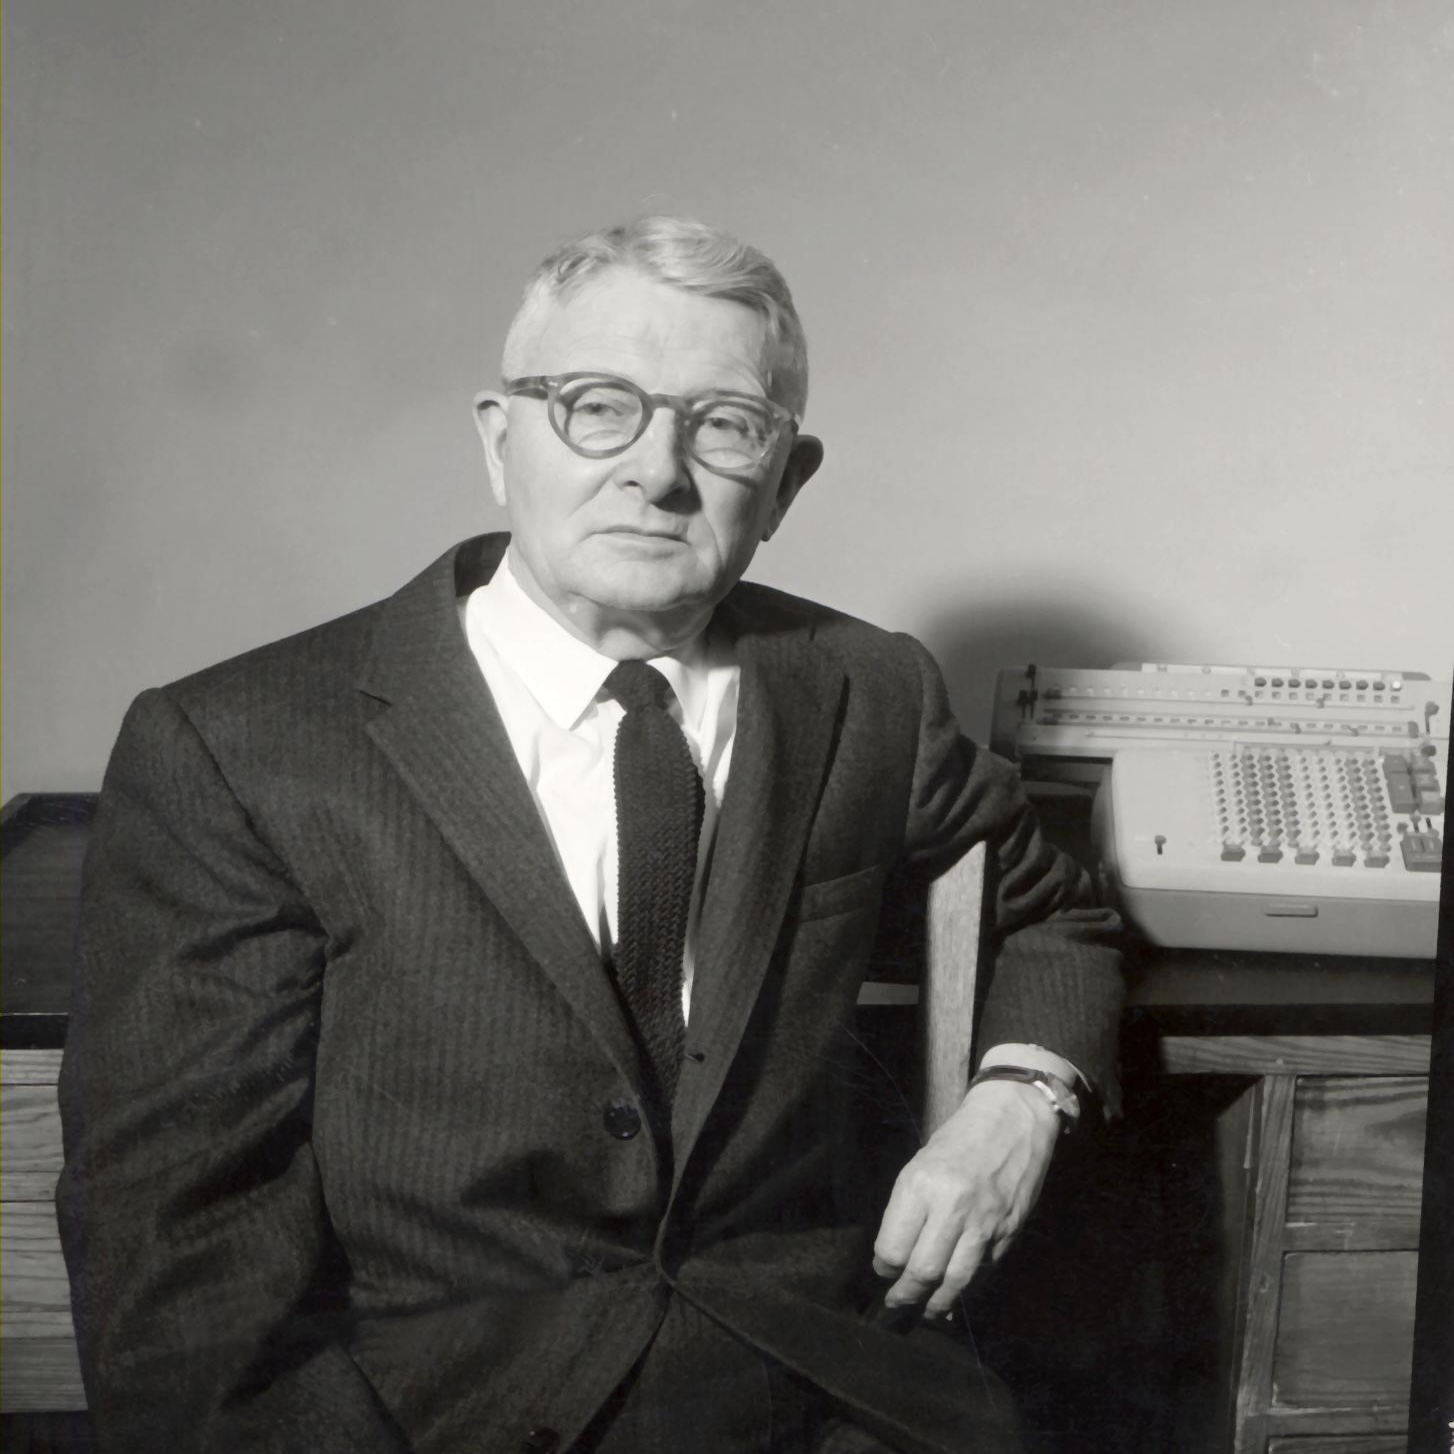
\includegraphics[width=\linewidth]{_wright.jpg}
    \end{figure}
    \column{0.25\textwidth}
    \begin{figure}
        \centering
        \footnotesize\textbf{Charles Spearman} \\
        \vspace{0.2em}
        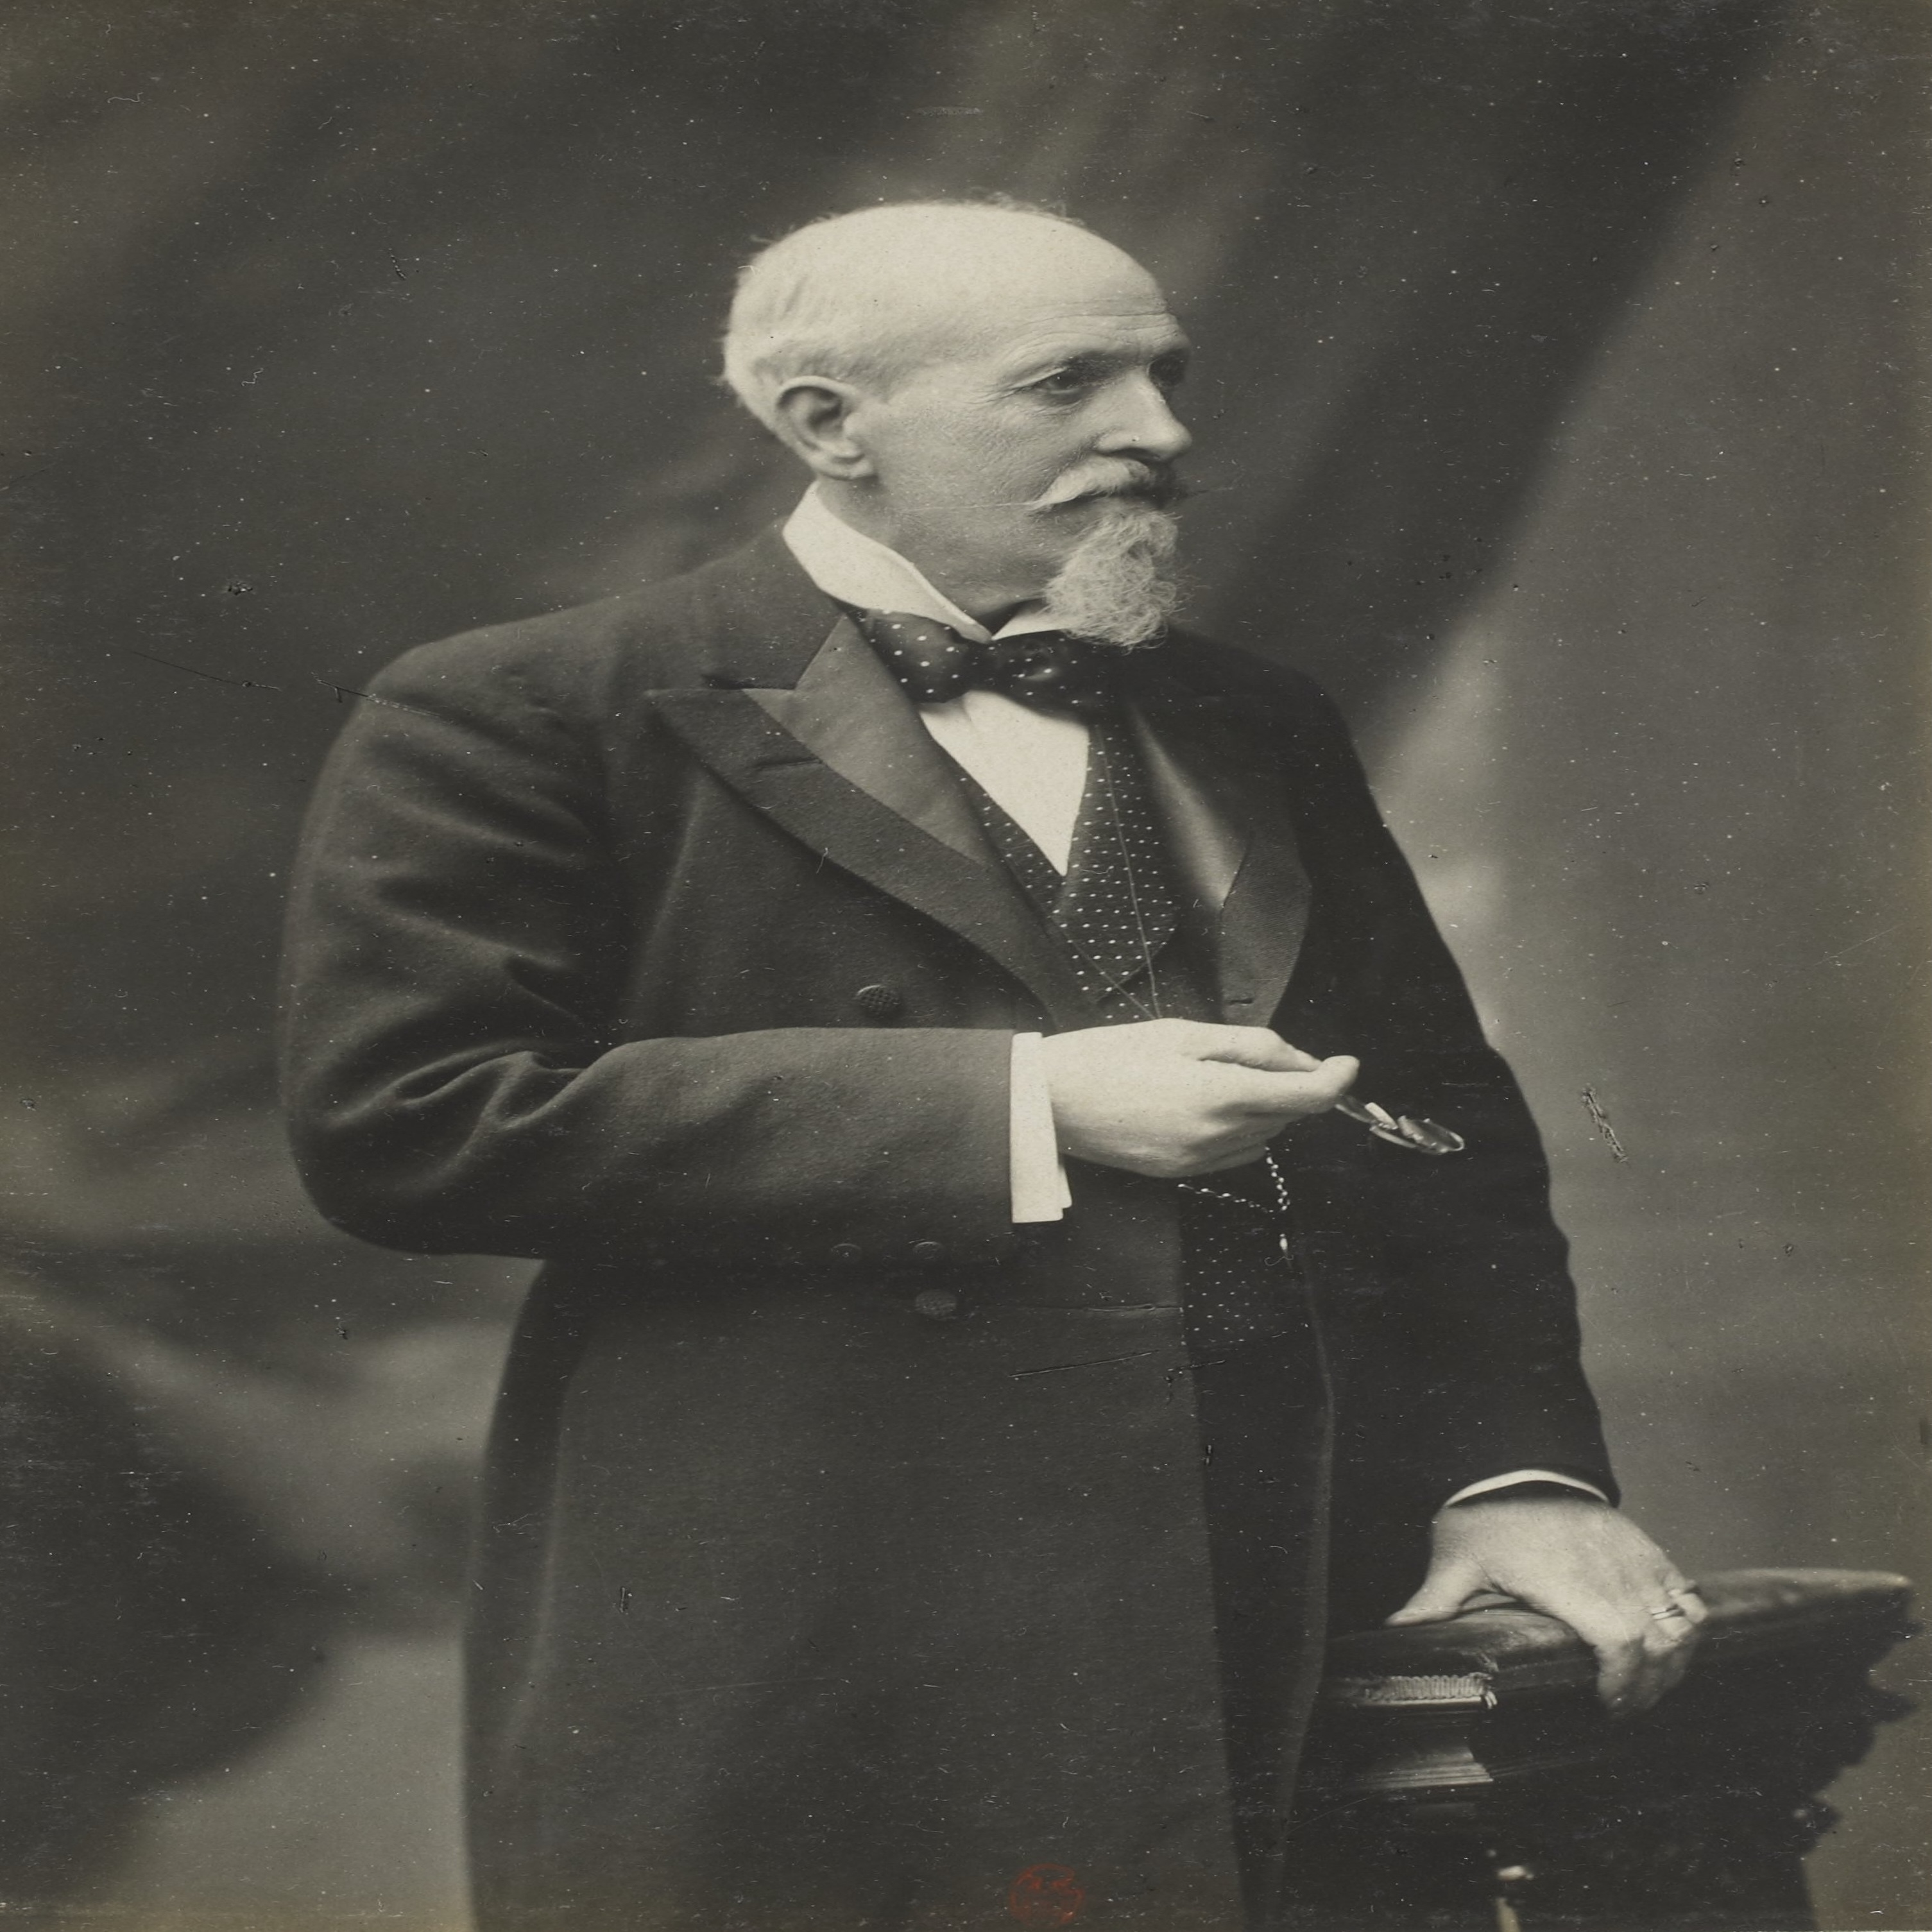
\includegraphics[width=\linewidth]{spea.jpg}
    \end{figure}
    \column{0.25\textwidth}
    \begin{figure}
        \centering
        \footnotesize\textbf{Louis Thurstone} \\
        \vspace{0.2em}
        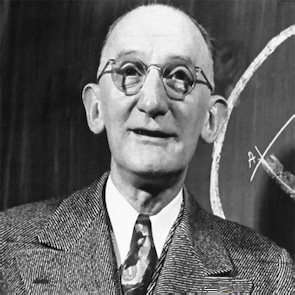
\includegraphics[width=\linewidth]{_thurstone.jpg}
    \end{figure}
    \column{0.25\textwidth}
    \begin{figure}
        \centering
        \footnotesize\textbf{Karl Jöreskog} \\
        \vspace{0.2em}
        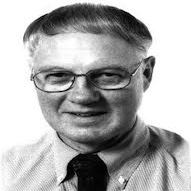
\includegraphics[width=\linewidth]{_joreskog.jpg}
    \end{figure}
  \end{columns}
\end{frame}

\begin{frame}{Brief history of SEM}
    \begin{block}{CB-SEM: Covariance-Based SEM}
        \begin{itemize}
            \item Formalised by Karl Jöreskog (1969) with LISREL;
            \item Objective: reproduce the observed \textbf{covariance matrix};
            \item Based on \textbf{maximum likelihood}.
        \end{itemize}
    \end{block}
    \begin{block}{PLS-SEM: Partial Least Squares SEM}
        \begin{itemize}
            \item Introduced by Herman Wold (1970s);
            \item \textbf{Component-based}, iterative approach;
            \item Focused on \textbf{maximising explained variance};
            \item Preferable in case of: small samples, formative models, non-normality.
        \end{itemize}
    \end{block}
\end{frame}

\section{A Bit of Theory}
\begin{frame}{Analysis process}
    SEM analysis goes through four phases, the same for both \textbf{CB-SEM} and \textbf{PLS-SEM}. However, the specific criteria to be used differ, as these models differ in their functioning and purposes (e.g. Reflective or Formative LVs). We will focus on the four phases of the process with an emphasis on \textbf{CB-SEM}: \\
    \vspace{1em}
    \begin{enumerate}
        \item Model specification
        \item Model identification
        \item Model estimation
        \item Model evaluation
    \end{enumerate}
\end{frame}

\begin{frame}{Model specification}
    \begin{block}{Phase 1:}
        The first phase consists of defining the theoretical model and the hypothesised relationships. In many software packages (including Stata) model specification can be done either by drawing diagrams or by writing code. \\
        \vspace{1em}
        \centering
        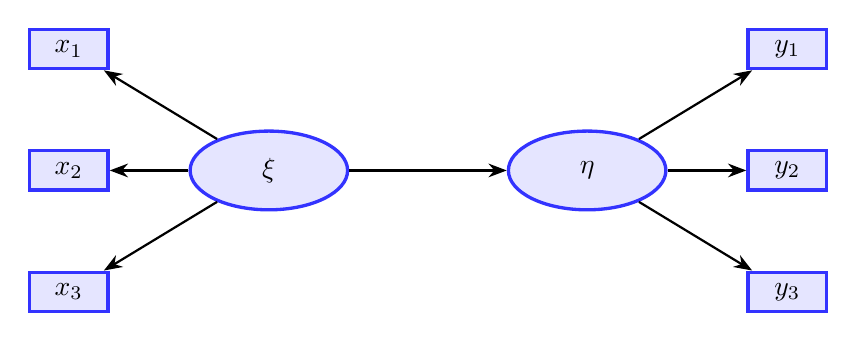
\begin{tikzpicture}
            \node[lv] (et) {$\eta$};
            \node[lv, left=2 of et] (xi) {$\xi$};
            \node[mv, left=of xi] (x2) {$x_2$};
            \node[mv, above=of x2] (x1) {$x_1$};
            \node[mv, below=of x2] (x3) {$x_3$};
            \node[mv, right=of et] (y2) {$y_2$};
            \node[mv, above=of y2] (y1) {$y_1$};
            \node[mv, below=of y2] (y3) {$y_3$};
            \draw[arrow] (xi) -- (et);
            \draw[arrow] (xi) -- (x1);
            \draw[arrow] (xi) -- (x2);
            \draw[arrow] (xi) -- (x3);
            \draw[arrow] (et) -- (y1);
            \draw[arrow] (et) -- (y2);
            \draw[arrow] (et) -- (y3);
        \end{tikzpicture} \\
        \vspace{1em}
        \small
        \texttt{. sem (Xi -> x1 x2 x3) (Eta -> y1 y2 y3) (Xi -> Eta)}
    \end{block}
\end{frame}

\begin{frame}{Model identification}
    \begin{block}{Phase 2:}
        Unfortunately, not everything that can be drawn can also be estimated. The \textbf{T-Rule}, for example, is a necessary (but not sufficient) condition for a model to be identifiable:
    \end{block}
    \[
    t \leq \frac{p(p+1)}{2}
    \]
    \begin{itemize}
        \item $t$ is the number of parameters to be estimated (arrows in the diagrams);
        \item $p$ is the number of manifest variables in the model.
    \end{itemize}
    \vspace{1em}
    \small
    \begin{itemize}
        \item If $t < \frac{p(p+1)}{2}$ the model is \textit{over-identified}: estimable and testable;
        \item If $t = \frac{p(p+1)}{2}$ the model is \textit{just-identified}: estimable but not testable (degrees of freedom = 0);
        \item If $t > \frac{p(p+1)}{2}$ the model is \textit{under-identified}: cannot be uniquely estimated.
    \end{itemize}
\end{frame}

\begin{frame}{Model identification}
    \centering
    $t \leq \frac{p(p+1)}{2}$ \hspace{1em} \textbf{?} \\
    \vspace{2em}
        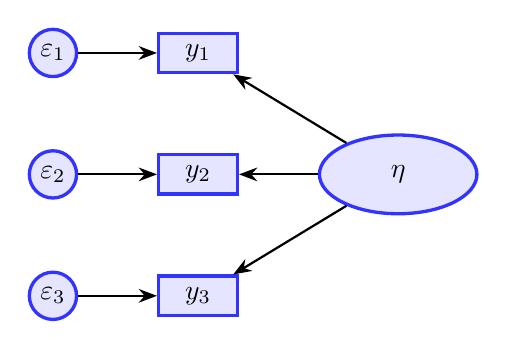
\begin{tikzpicture}
            \node[lv] (l) {$\eta$};
            \node[mv, left=of l] (x2) {$y_2$};
            \node[mv, above=of x2] (x1) {$y_1$};
            \node[mv, below=of x2] (x3) {$y_3$};
            \draw[arrow] (l) -- (x1);
            \draw[arrow] (l) -- (x2);
            \draw[arrow] (l) -- (x3);
            \pause
            \node[ev, left=of x1] (e1) {$\varepsilon_1$};
            \node[ev, left=of x2] (e2) {$\varepsilon_2$};
            \node[ev, left=of x3] (e3) {$\varepsilon_3$};
            \draw[arrow] (e1) -- (x1);
            \draw[arrow] (e2) -- (x2);
            \draw[arrow] (e3) -- (x3);
        \end{tikzpicture}
\end{frame}

\begin{frame}{Model estimation}
    \begin{block}{Phase 3:}
        Model estimation consists of calculating the parameter values that best reproduce the observed covariance matrix (typically through \textit{maximum likelihood}).
    \end{block}
\end{frame}

\begin{frame}{Model evaluation}
    \begin{block}{Phase 4:}
        Model evaluation takes place at three levels:
        \begin{enumerate}
            \item \textbf{Global goodness of fit}:
            \begin{itemize}
                \item $\chi^2$ test (preferably non-significant)
                \item RMSEA $< 0.06$
                \item CFI, TLI $> 0.95$
                \item SRMR $< 0.08$
            \end{itemize}
            \item \textbf{Measurement model}:
            \begin{itemize}
                \item $\lambda_i$ (factor loadings) $> 0.5$ and significant
                \item CR (Composite Reliability) $> 0.7$
                \item AVE (Average Variance Extracted) $> 0.5$
                \item Discriminant validity (e.g. Fornell-Larcker criterion)
            \end{itemize}
            \item \textbf{Structural model}:
            \begin{itemize}
                \item $\beta$ (path coeff.) significant
                \item Acceptable $R^2$ for endogenous variables
                \item Significant direct, indirect and total effects (if relevant)
            \end{itemize}
        \end{enumerate}
    \end{block}
\end{frame}

\begin{frame}{Modification Indices}
    \begin{block}{What are they?}
        \textbf{Modification Indices} (MI) signal potential improvements to the model by introducing unspecified parameters (e.g. residual covariances).
    \end{block}
    \vspace{1em}
    \textbf{Caution:} suggested modifications should be accepted only if theoretically justified, to avoid \textit{overfitting}.\\
    \vspace{1em}
    By introducing new parameters to be estimated, we go back to Phase 1!
\end{frame}

\end{document}
